\documentclass{report}
\usepackage{svg}
\usepackage{float}
\usepackage{etoolbox}% http://ctan.org/pkg/etoolbox
\usepackage{enumitem}% http://ctan.org/pkg/enumitem
\usepackage{hyperref}
\hypersetup{
	colorlinks,
	linkcolor={black!50!blue},
	citecolor={blue!50!black},
	urlcolor={blue!80!black}
}

\usepackage{tikz}
\usepackage{circuitikz} %Circuit drawing tools
\usepackage{siunitx}
\usepackage{multirow}
\usepackage{graphicx}

\usepackage{listings}
\usepackage{color}
\usepackage{amsmath}
\usepackage{cancel}
\usepackage[margin=1in]{geometry}

\usepackage[toc,page]{appendix}
\setcounter{tocdepth}{4}
\setcounter{secnumdepth}{5}
\usepackage{tocbibind}


\usepackage{fancyhdr}
\setlength{\headheight}{13.6pt}
\fancyhf{}
\fancyhead[L]{UMSATS Altium Guide}
\fancyhead[R]{\rightmark}
\fancyfoot[R]{v0.2}
\fancyfoot[C]{\thepage}
\pagestyle{fancy}


\begin{document}
	\begin{titlepage}
		\centering
		\includegraphics[width=0.7\textwidth]{"pics/logo"}\par\vspace{1cm}

		\vspace{1cm}

		\vspace{1.5cm}
		{\huge\bfseries Altium Guide\par}
		\vspace{2cm}
		{\Large\itshape UMSATS\par}
		\vfill

		Author:\\ Aleksa Svitlica
		\par		
		\vfill
		
		{\large Last Updated: March 18, 2018\par}
	\end{titlepage}
	\pagenumbering{roman}
	\tableofcontents
	\listoffigures
	\newpage
	\pagenumbering{arabic}
	\chapter{Getting Started}
	First two important notes:
	\begin{enumerate}
		\item I am using Altium Designer 17.1
		\item I am writing this as I learn Altium so expect mistakes. If something seems wrong it probably is.
	\end{enumerate}

	\section{Creating a new PCB project}
	\begin{itemize}
		\item File-$>$New-$>$Project...
		\item Select PCB project from the project types options on the left side.
		\item For project templates simply choose $<$Default$>$ because we will be importing a STEP file later.
	\end{itemize}
	If Altium is giving you errors when you try to create a new project that probably means you haven't selected a valid license. To fix this you can select View-$>$Home to open up the Home page. Then click on the Admin tab, make sure you are logged in and select a license from below.
	\section{Create a PCB file}
	Click File-$>$New-$>$PCB. This should result in a screen like below:
	
	\begin{figure}[H]	
		\centering
		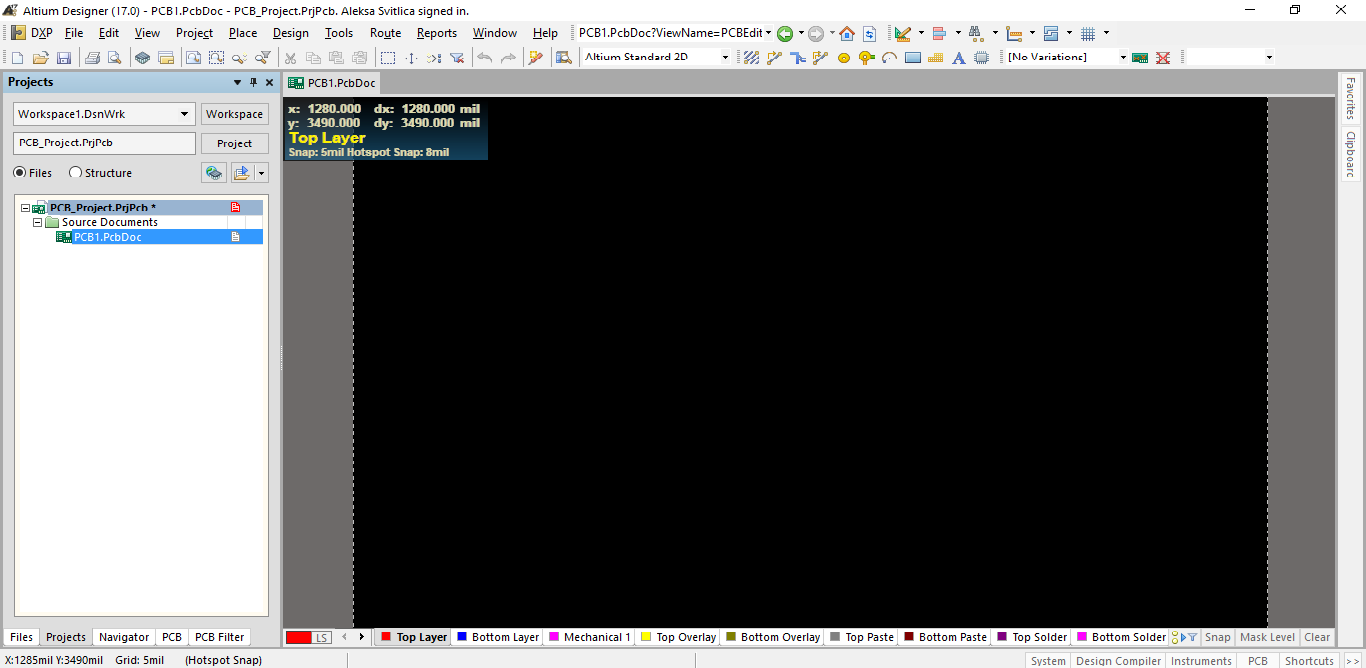
\includegraphics[width=16cm, height=8cm]{pics/new_pcb_file.png}
		\caption{New PCB file.}
		\label{fig 1}
	\end{figure}
	The next step is import our step file and use that to create the physical PCB shape. To do this first click 3 to switch to 3D mode, you can switch between 2D and 3D by pressing 2 or 3. Then click Place-$>$3D Body to bring up a new menu. In this menu there are a couple things we need to change:
	\begin{itemize}
		\item 3D Model Type: Select Generic 3D model
		\item Further down the window there will now be an option to select a file to import for the generic 3D model. Select embedded and then choose the correct STEP file provided to you by the mechanical team.
		\item After loading your STEP file there should be a model displayed in the window, if it looks like a horizontal line don't worry, we just need to rotate it. In rotation x simple put 90 or -90.
	\end{itemize}
	\begin{figure}[H]	
		\centering
		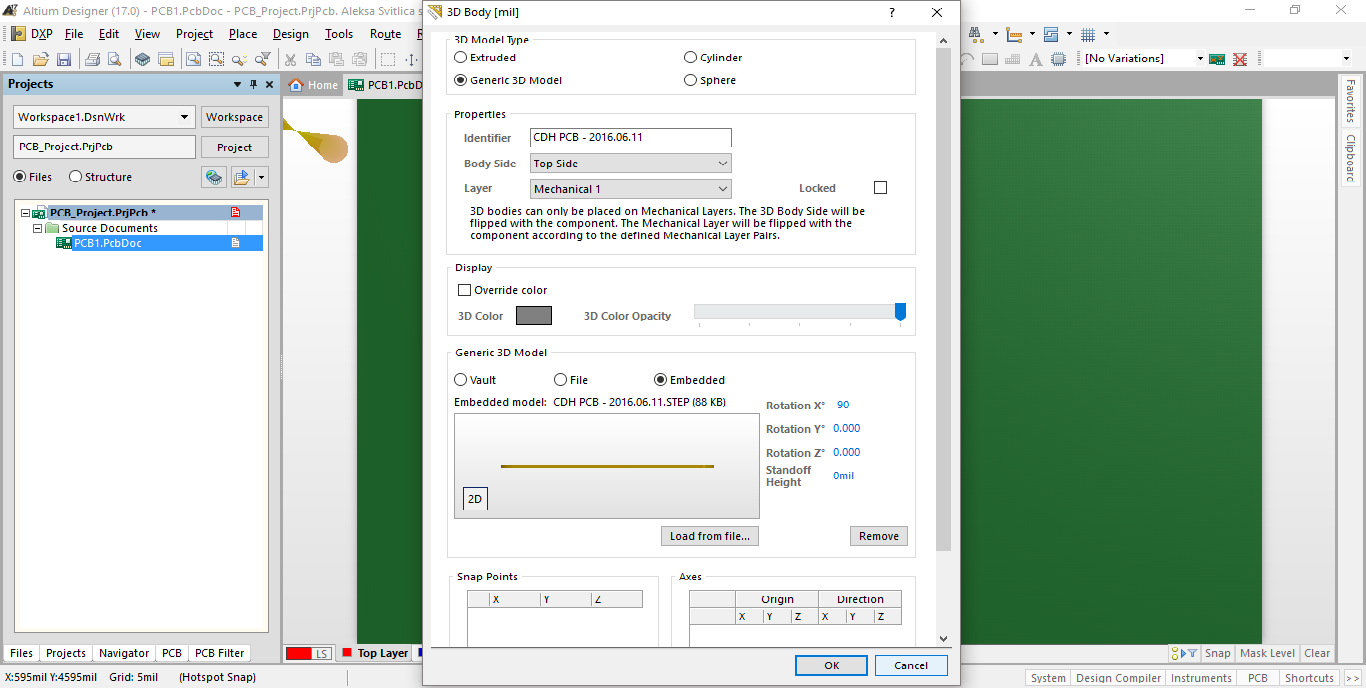
\includegraphics[width=16cm, height=8cm]{pics/import_step.png}
		\caption{Importing STEP file as 3D body.}
		\label{fig 2}
	\end{figure}
	Click OK and left click again to place your 3D body down, where you place it doesn't matter for now.
	\begin{figure}[H]	
		\centering
		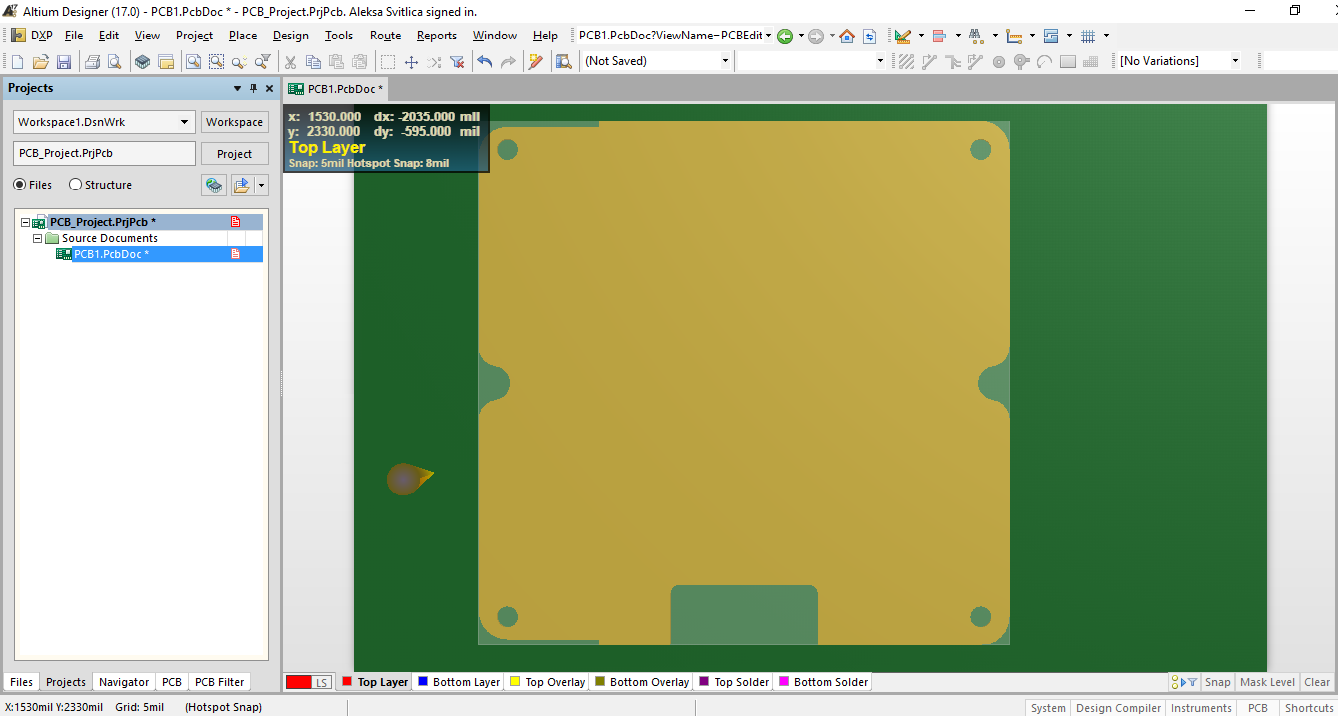
\includegraphics[width=16cm, height=8cm]{pics/3d_body_pic1.png}
		\caption{Placing 3D body.}
		\label{fig 3}
	\end{figure}
	Now to make your PCB match this 3D body go to Design-$>$Board Shape-$>$Define From 3D Body. If this is option is unclickable for you make sure you are in 3D mode and try again. Your cursor should look like a + symbol and that window which says Top Layer in bold yellow words should also say Pick a 3D Body.
	\begin{figure}[H]	
		\centering
		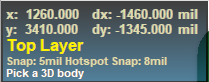
\includegraphics[width=8cm, height=4cm]{pics/pick_3d_body.png}
		\caption{Pick 3D body.}
		\label{fig 4}
	\end{figure}
	Click on the 3D body you just placed, the words in that window should now say select face, click again on the 3D body. It will open up a couple windows, just click cancel or closed until you see the following screen.

	\begin{figure}[H]	
		\centering
		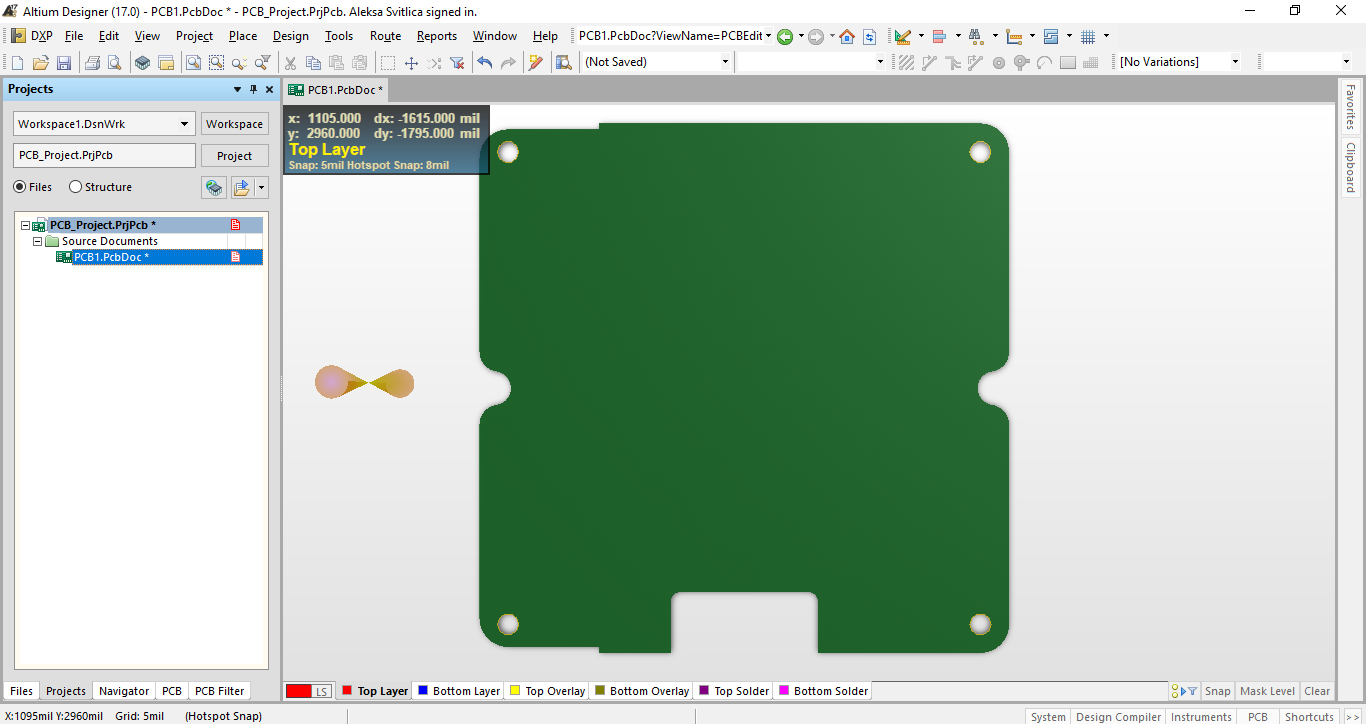
\includegraphics[width=16cm, height=8cm]{pics/3d_body_pic2.png}
		\caption{Finished placing 3D body.}
		\label{fig 5}
	\end{figure}

	The PCB shape is now defined, we are ready to define layers.
	
	\section{Layer Stack Manager}
	To access the layer stack manager, select Design-$>$Layer Stack Manager. Here you can define each layer of your PCB, it will default to a 2 layer setup. Even though you see a bunch of layers listed, only the copper layers actually count when we say 2-layer board. I can't offer any suggestions about how many layers you should use, what thickness or what material since this is a topic I know almost nothing about. For reference I've included a picture of the 4-layer subsystems board that Mike Lambeta designed.
	
	\begin{figure}[H]	
		\centering
		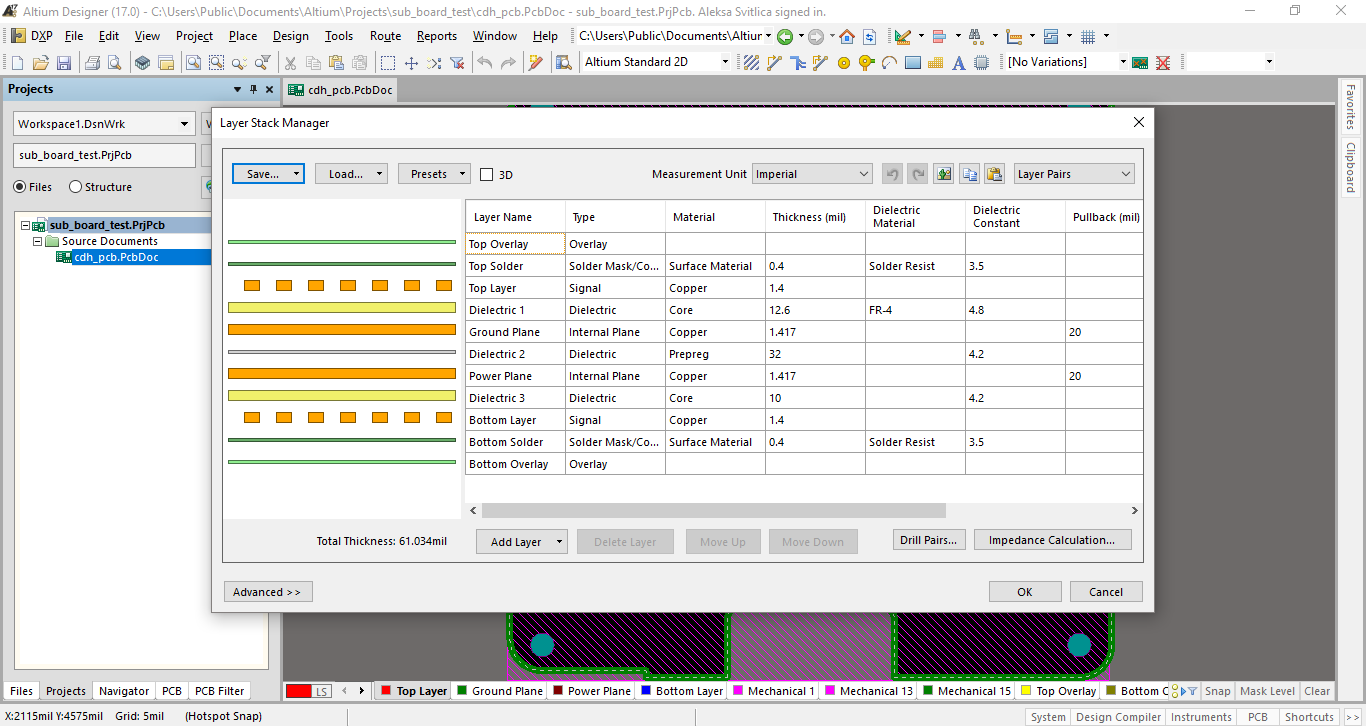
\includegraphics[width=16cm, height=8cm]{pics/layer_stack.png}
		\caption{Layer stack manager.}
		\label{fig 6}
	\end{figure}
	
	\chapter{Parts Libraries}
	\section{Importing Libraries}
	I would recommend downloading the libraries Altium provides on their \href{http://techdocs.altium.com/display/ADOH/Download+Libraries}{website}. It is much easier to work with preexisting models since making components is a hassle. You can store the libraries anywhere on your computer and import the ones you need in your project. Click on Place-$>$Part... and then select Choose. This will bring up a menu like in figure \ref{fig 7}, click on the three dots to the left of find to bring up the library import menu. After importing, the libraries will be selectable in the menu seen below and individual parts can be selected.
	\begin{figure}[H]	
		\centering
		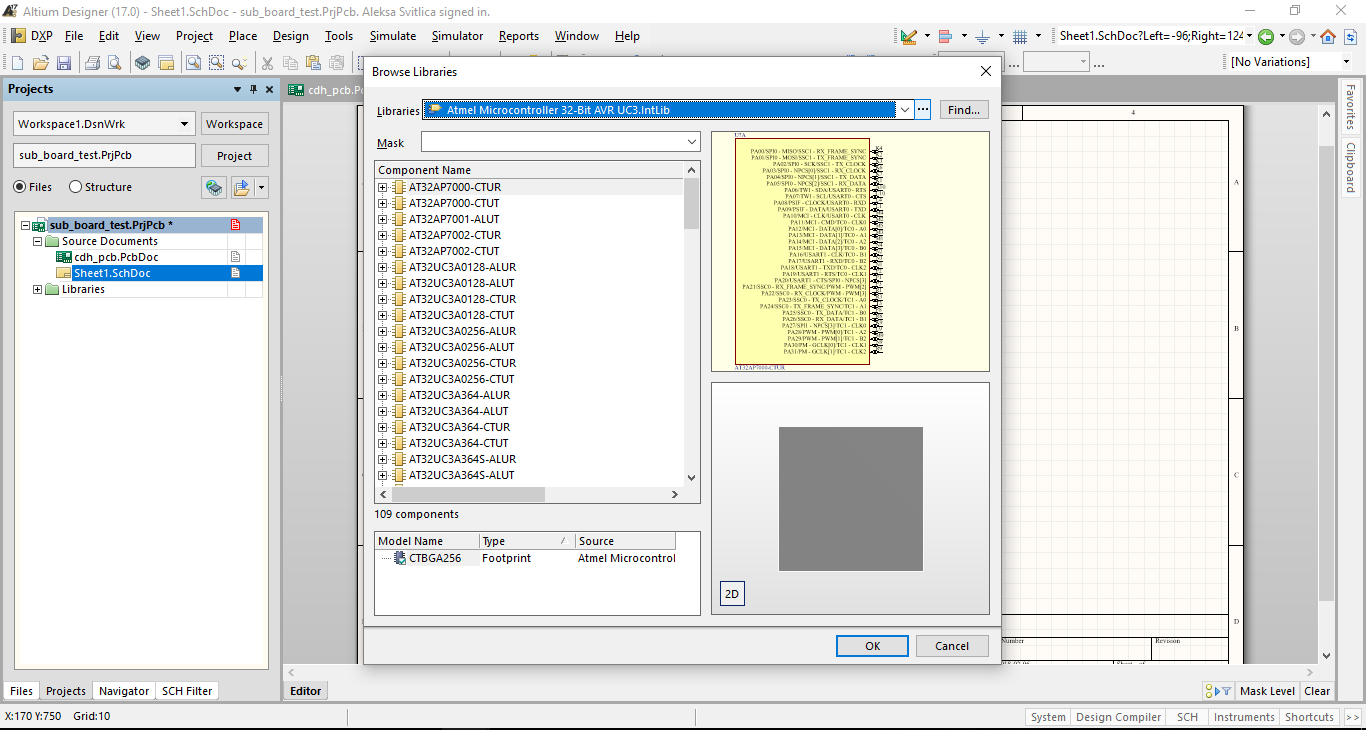
\includegraphics[width=16cm, height=8cm]{pics/library.png}
		\caption{Browsing libraries.}
		\label{fig 7}
	\end{figure}

	Note: The link to the Altium libraries is not exhaustive, it is simply a collection of common libraries used and may not have the components you need. For most of the components I used I Googled "Altium component-name-here" which lead to a designcontent.live.altium.com website. In the libraries found this way you can scroll through and make sure your component is included in the library.

	\section{Custom Components [TODO]}
	All the information I have on this topic came from this \href{https://www.youtube.com/watch?v=ozKoxXyzHC8}{video}.\\\\
	To add a new library to your project, right click on the PrjPCB file in the projects tab on the left. Navigating through the menu like in the picture below you will see an option to add a new Schematic Library and a PCB Library. Essentially the PCB Library defines the footprint of the component, the physical dimensions, pad placement and orientation references on the PCB. The Schematic library is where you define the pins, input/output and anything you would need when using it in a schematic. As the naming suggests, the PCB Library defines what we see when importing that component in the PCB file; the Schematic Library defines what we see when importing the component into a schematic.
	\begin{figure}[H]	
		\centering
		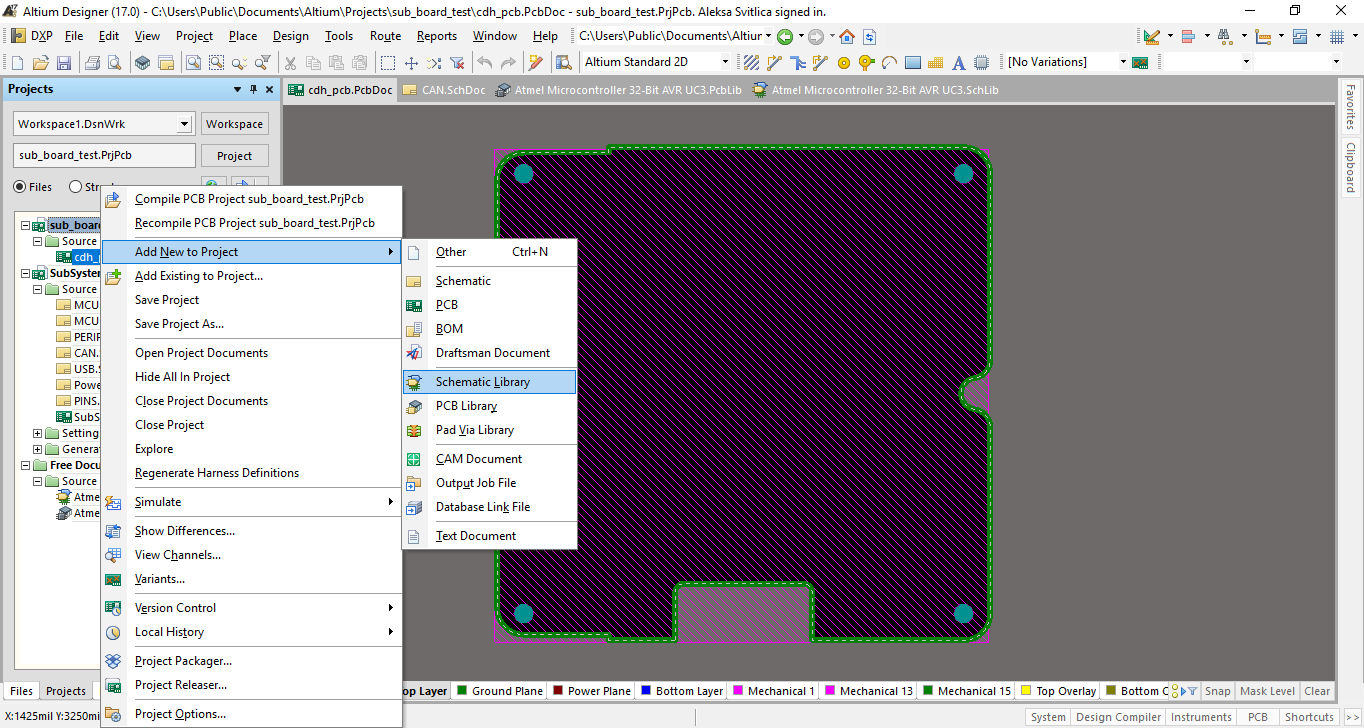
\includegraphics[width=16cm, height=8cm]{pics/new_schematic_menu.png}
		\caption{Menu for adding new schematic library.}
		\label{fig 8}
	\end{figure}
	\subsection{PCB Libraries [TODO]}
	All the information needed to create a PCB footprint is located in the component datasheet. The bare minimum you need to define is the pads or holes needed to mount the component.
	\subsubsection{Creating Holes/Pads}
	Pins and pads should be the first thing created in a PCB footprint. They are created using the same tool, Place->Pad. It will default to a hole but this can be changed by modifying the properties (figure \ref{pad_menu}). The name should match the numbers in the datasheet to avoid confusion. To create a pad for surface mount components select Top Layer in the Layer property. Doing so will automatically change the hole size to 0 and likely change the pad color to red. An important thing to keep track of is the dimensions, datasheets will alternate between milimeters (mm) and thousandth of an inch (mil); Altium defaults to mils.
	
	\begin{figure}[H]	
		\centering
		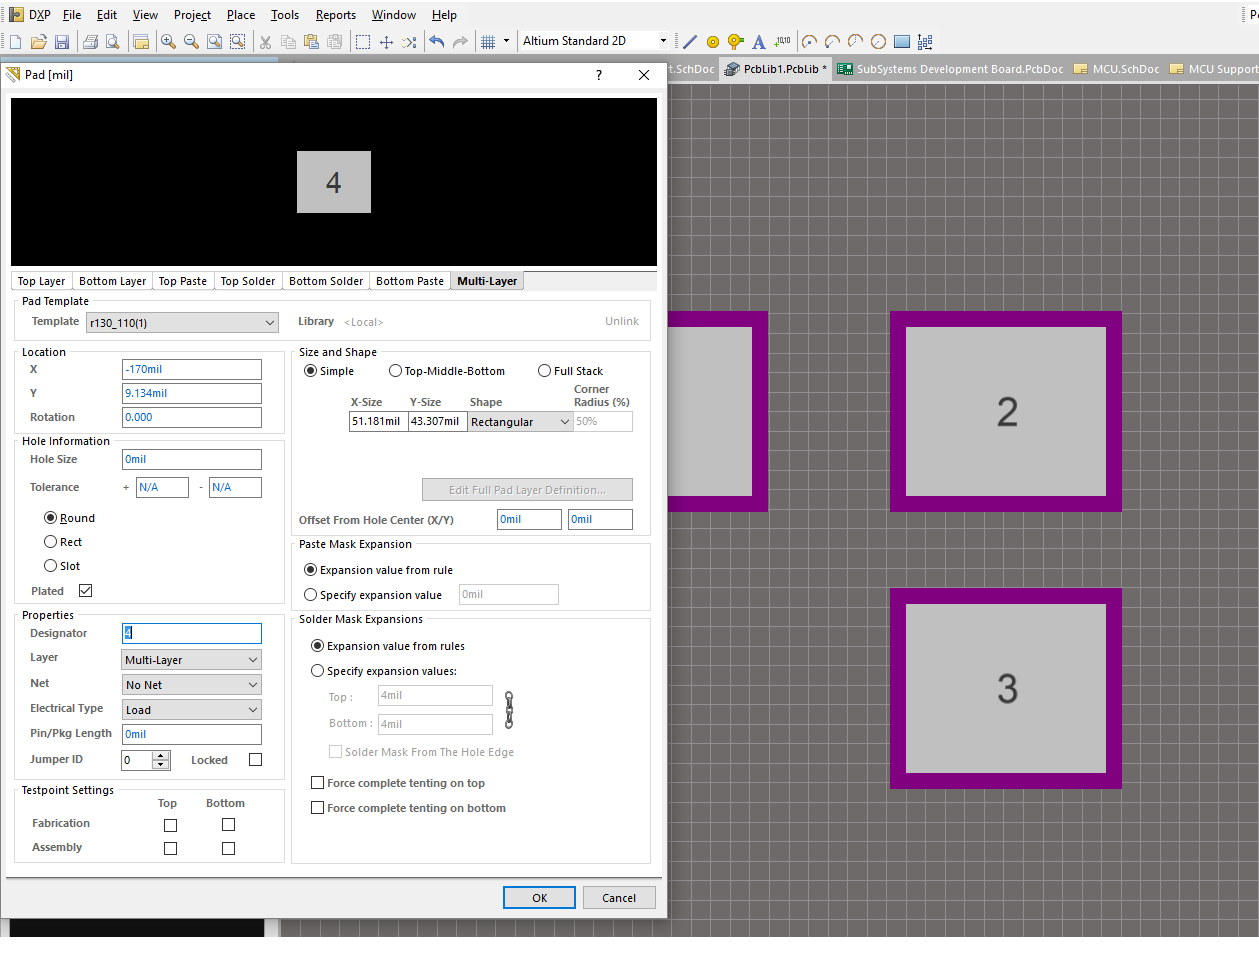
\includegraphics[width=16cm, height=8cm]{pics/pad_creation.png}
		\caption{Pad properties.}
		\label{pad_menu}
	\end{figure}

	Notes: To ensure correct positioning of pads relative to each other I used the location property of the pads. If creating holes, it is recommended to use the max hole diameter (in the datasheet) plus 0.25mm to ensure easy installation.
	
	\subsubsection{Defining the Outline[TODO]}
	\subsubsection{3D Body[TODO]}
	\subsection{Schematic Libraries}
	The core requirement in schematic libraries is the pins. These pins need to match up with the holes or pads created in the component footprint (PCB library). Creating a pin can be done through the Place menu or the toolbar. The space bar rotates the pin. After placing a pin you will need to set the properties in the menu shown in figure \ref{pin_creation}. Display name can be anything but ideally describes what the pin is for. Designator must be a number which matches a hole or pad in the footprint. To add the footprint click the Add Footprint button on the bottom of the screen and select the footprint you made previously.
	\begin{figure}[H]	
		\centering
		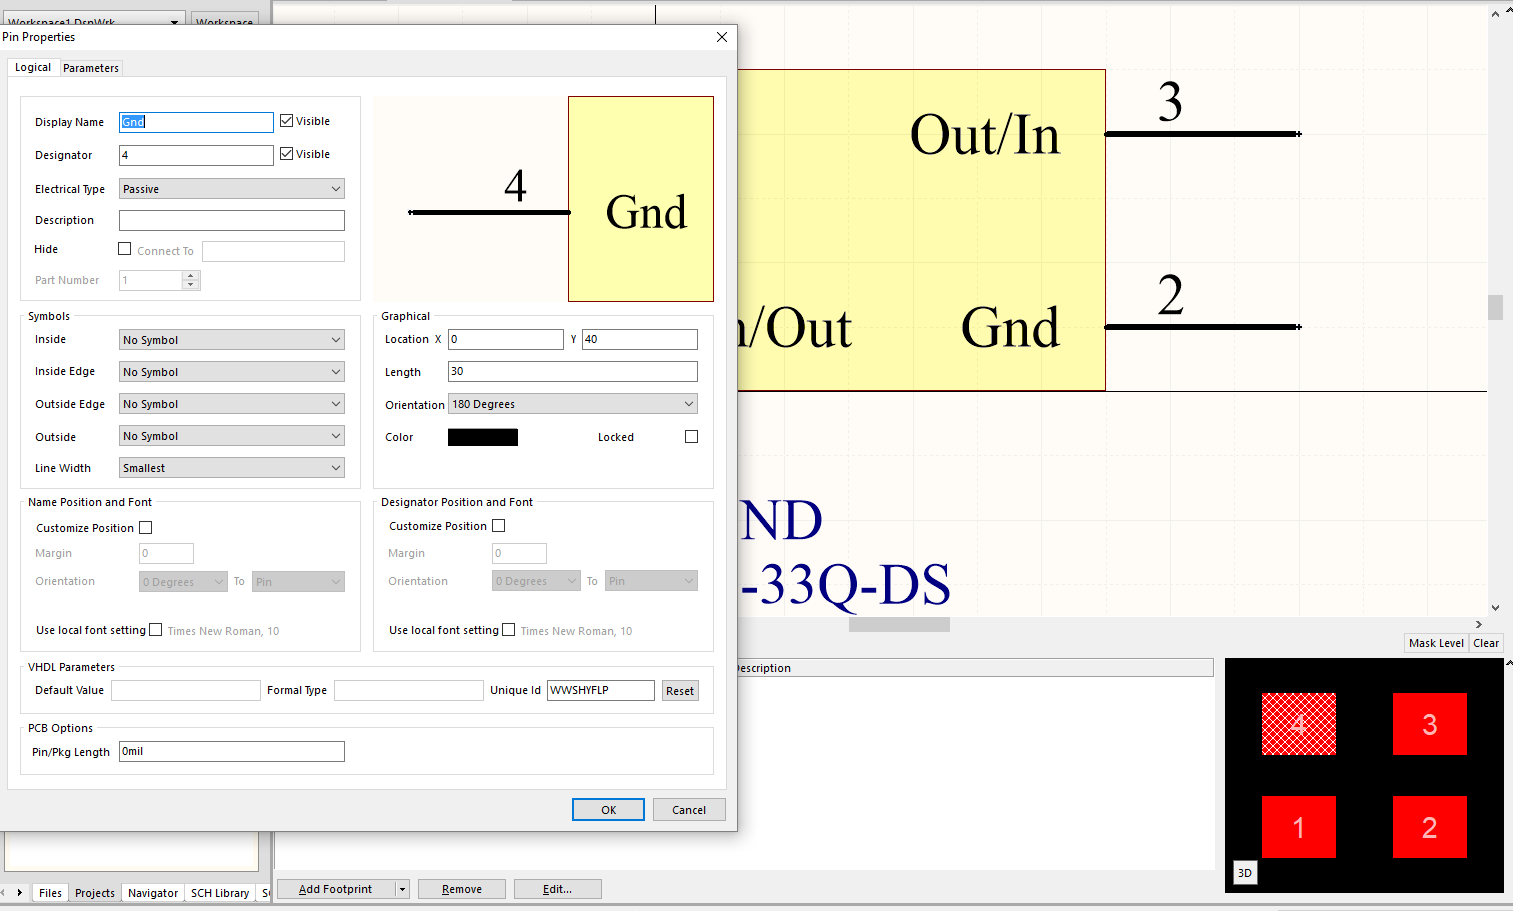
\includegraphics[width=16cm, height=8cm]{pics/pin_creation.png}
		\caption{Modifying pins.}
		\label{pin_creation}
	\end{figure}
	If possible it is best to place one a symbol to represent your component. If you don't have the symbol and it isn't provided by Altium, a common alternative is to place a rectangle between your pins like in figure \ref{schem_lib}.
	\begin{figure}[H]	
		\centering
		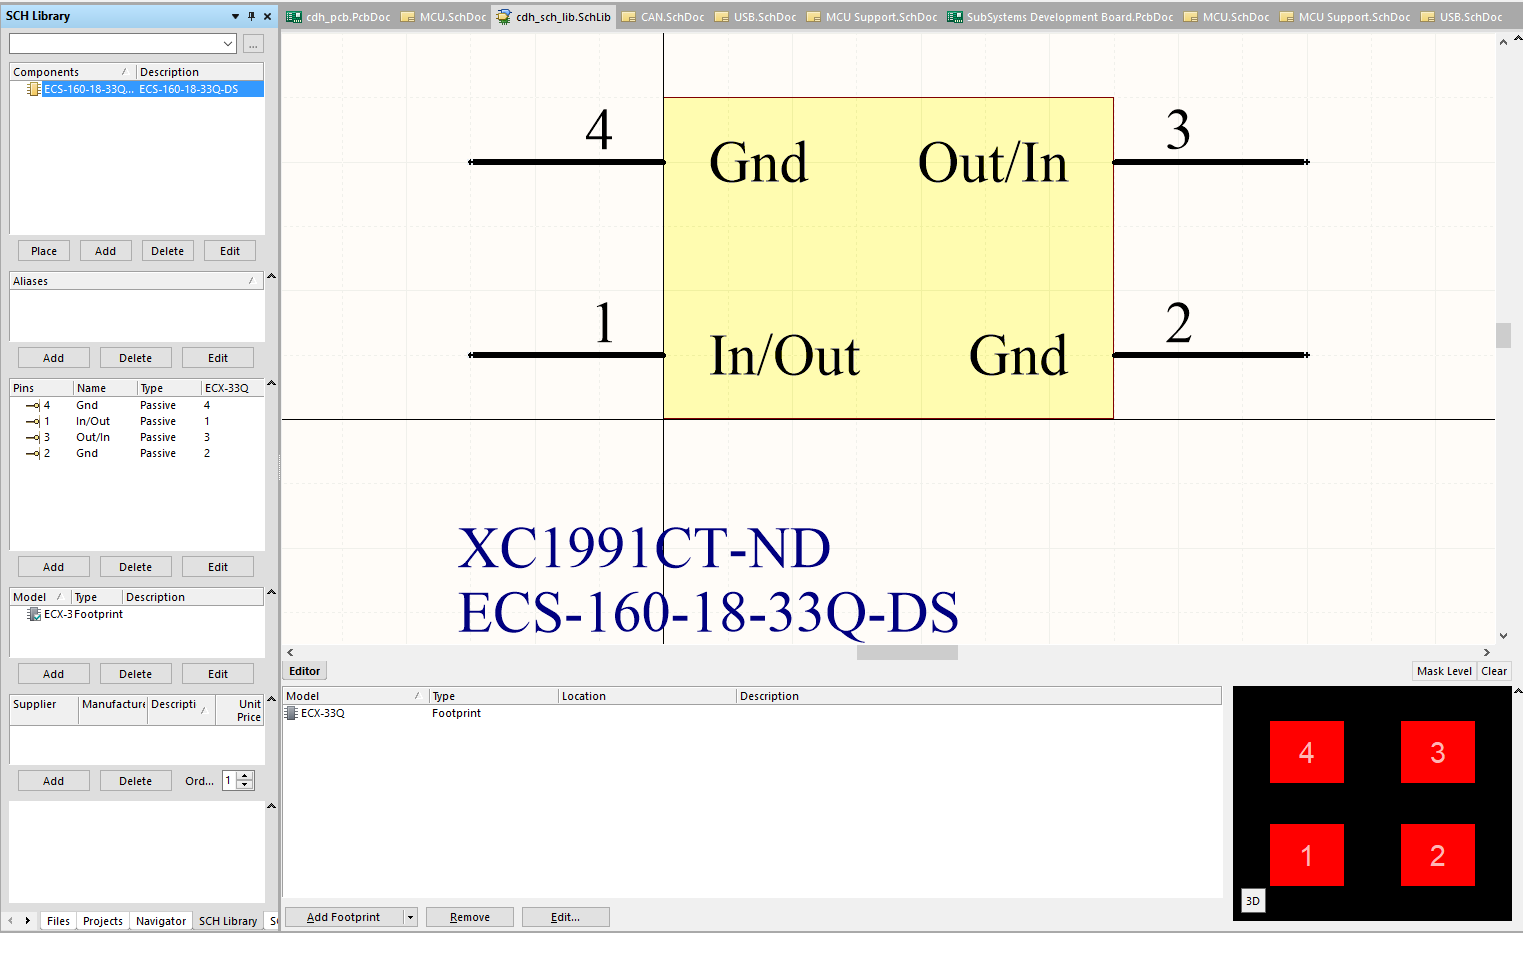
\includegraphics[width=16cm, height=8cm]{pics/schem_lib1.png}
		\caption{Sample schematic library.}
		\label{schem_lib}
	\end{figure}
	When finished making the component it is time to add additional properties and useful information. Click on the SCH Library tab on the bottom left to open up the component menu seen in figure \ref{schem_lib}. Click on the component you just created and select edit. This will bring up a menu like in figure \ref{schem_lib_properties}. The designator field should have some standard letters followed by a question mark (R for resistor, C for capactior, U for microcontroller etc.). The comment and description fields are up for interpretation. I personally put a colloquial description in the comment and then copy the description from Digikey for the description. The parameters on the right side of the menu are also freeform in their use. In general you want to put information which will make it easier for other people to get information about this component. I opted to include the Digikey and manufacturer part numbers.

	\begin{figure}[H]	
		\centering
		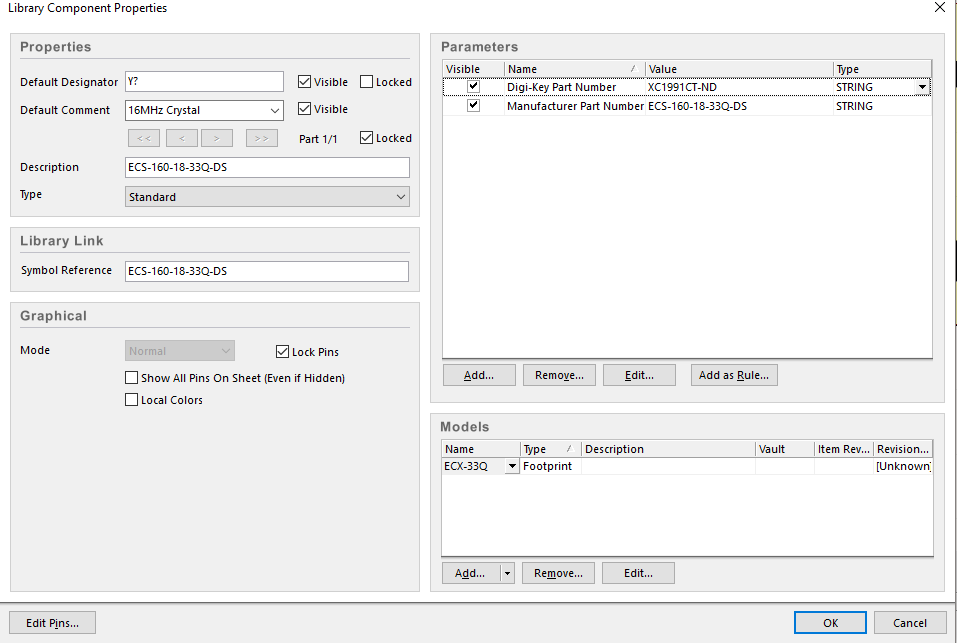
\includegraphics[width=16cm, height=8cm]{pics/schem_lib2.png}
		\caption{Library component properties.}
		\label{schem_lib_properties}
	\end{figure}
	
	\newpage
	
	\chapter{Making Schematics}
	Before making any schematics, there should be some planning in regards to how components will be grouped. Unless you are designing a simple PCB with very few components, it will be useful to create multiple schematics. For example, in the subsystems development board there are seven schematics: MCU, MCU Support, Peripherals, CAN, USB, Power and Pins.
	
	\section{Placing Components}
	Click on Place-$>$Part... and select Choose. This will bring you to the menu in figure \ref{fig 7}, there you can select libraries and components from those libraries.
	\subsection{Placing the MCU}
	I chose to start with the MCU because everything will branch off this component. I selected the Atmel Microcontroller AVR UC3.IntLib library I downloaded earlier and searched by the component name in the mask field, AVRUC3C2512C and then select the A2UT version of this component. After clicking Ok this will take you back to the schematic file where you can left click to place the component. The MCU is a special case in component placement because most of them are divided up into smaller parts to place on the schematic. When you left click, the next component queued for placement will look slightly different, keep clicking and placing on the schematic until you notice the components are starting to repeat. Alternatively, you can check with the identifier on the top left of the component, probably U?A, and keep placing until you notice that the identifier has reached U?A again. To stop placing components press the esc key. My placement can be seen in figure \ref{fig 9}. While the entire MCU is currently in the same schematic, I will be moving parts of it to separate schematics where it makes sense.
	
	\begin{figure}[H]	
		\centering
		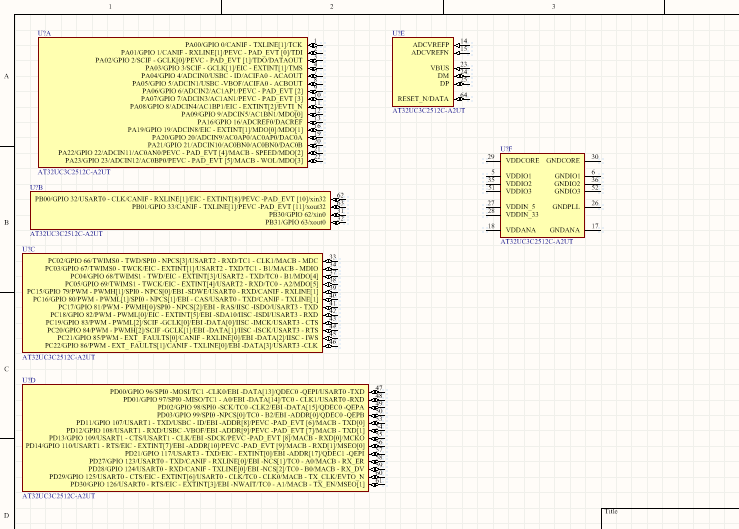
\includegraphics[width=16cm, height=8cm]{pics/mcu_place.png}
		\caption{Placing the MCU}
		\label{fig 9}
	\end{figure}
	Most other components are much simpler to place because they won't be divided up into smaller sections.
	
	\subsection{Placing Other Components}
	\begin{figure}[H]	
		\centering
		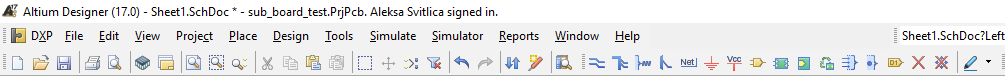
\includegraphics[width=16cm]{pics/schematic_toolbar.png}
		\caption{Schematic toolbar}
		\label{fig 10}
	\end{figure}
	\subsubsection{Ground and Voltage}
	Figure \ref{fig 10} shows the toolbar available when placing components on a schematic. Ground and voltage are both options on the toolbar, identified by their standard symbols. When placing a voltage source, it will default to Vcc, to change this right click and select properties. The net property is the label shown on the schematic.
	\subsubsection{Resistors, Capacitors and Inductors}
	In general, the resistors, capacitors and inductors you need can be taken from the standard parts library Miscelaneous Device.IntLib. The only reason to create custom components here would be to use a footprint that isn't included in the standard parts library.
	\subsection{Adding Ports}
	Ports are a tool than can be used to define I/O as input, output or bidirectional. These are used on the MCU pins to allow cleaner schematics. Rather than wiring the MCU directly to the rest of the schematic, we instead add ports to each MCU pin. Each port needs to have a name and an I/O type, these are defined after placing the port by right right clicking at selecting properties. For the MCU all ports should be bi-directional because we are going to place a matching port elsewhere to be used in the schematic.
	\begin{figure}[H]	
		\centering
		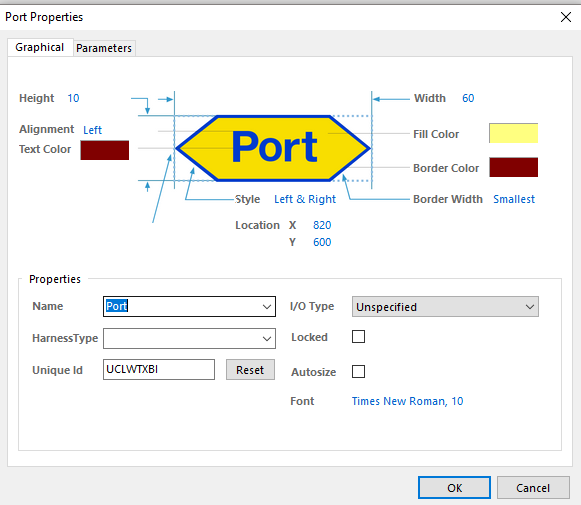
\includegraphics[width=16cm]{pics/port_menu.png}
		\caption{Port properties}
		\label{port menu}
	\end{figure}
	
	\chapter{Routing}
	
\end{document}